%%%%%%%%%%%%%%%%%%%%%%%%%%%%%%%%%%%%%%%%%%%%%%%%%%%%%%%%%%%%%%%%%%%%%%%%%%%%%%%%%%%%%%%%%%%%%
%									Chapitre 1												%
%%%%%%%%%%%%%%%%%%%%%%%%%%%%%%%%%%%%%%%%%%%%%%%%%%%%%%%%%%%%%%%%%%%%%%%%%%%%%%%%%%%%%%%%%%%%%
\chapter{Etat de l'art}
	\citationChap{
	If I knew how I knew everything I knew, then I would only be able to know half has much, because it will all be clogged up with where I know it from. So I cannot always cite my sources, I'm sorry.
	}{David Mitchell}
	\minitoc
	\newpage

%%%%%%%%%%%%%%%%%%%%%%%%%%%%%%%%%%%%%%%%%%%%%%%%%%%%%%%%%%%%%%%%%%%%%%%%%%%%%%%%%%%%%%%%%%%%%



% Début du chapitre


\section{Contexte}

	Depuis les premiers pas de l'informatique, une question s'est posée : est-ce que les machines peuvent penser ? \cite{turing1950computing} Cette question, bien qu'abstraite dans sa formulation, se réfère à l'intelligence humaine. Il n'est en effet ici pas question de savoir si ce que les ordinateurs font est de la pensée, mais bien si l'on peut reproduire l'intelligence humaine dans un cerveau électronique. Cet question a été le fondement d'un nouveau domaine scientifique qui a été nommé quelques années plus tard, lors de la conférence de Dartmouth \cite{mccarthy1955proposal} : l'intelligence artificielle.

	Les années qui suivirent n'amenèrent pas de résultats au niveau des espérences des chercheurs. Le domaine était encore trop limité par la puissance limitée des ordinateurs et les modèles primitifs n'arrivaient qu'à résoudre des tâches simples.

	La première évolution majeure est arrivée dans les années 90, lorsque les processeurs on dépassé le million de transistor par puce et lorsque les méthodes algorithmiques étaient plus avancées, avec par exmple la recherche rapide dans une bases de données. Ces changements on permis aux modèles d'IA d'exploiter plus de données, plus rapidement et avec uoù la programmation et les heuristiques étaient les facteurs les plus importants de réussite. Les succès les plus connus de cette époque comptent la victoire de Deep Blue sur Kasparov aux échecs \cite{campbell2002deep}, et le programme Watson d'IBM \cite{ferrucci2012introduction}, qui pourrait être considéré comme le dernier grand projet d'IA de cette période. Il commençait déjà à utiliser quelque chose qui allait constituer la nouvelle évolution de l'IA : l'apprentissage.

	L'apprentissage automatique est une sous-discipline du domaine de l'IA qui s'est développé tout au long de son histoire et qui est passé sur le devant de la scène depuis les années 2010. C'est une combinaison de plusieurs facteurs qui l'on amené à dépasser tous les records à ce moment là : les réseaux de neurones multicouches étaient arrivés à maturation et permettaient l'apprentissage de données avec des représentations à haut niveau d'abstraction. Les dispositifs de calculs étaient toujours plus puissants, avec notamment les cartes graphiques dédiées devenues programmables et qui permirent d'effectuer du calcul de nombres à virgule flottante en parallèle. Et en dernier, la présence de jeux de données massifs avec lesquels on pouvait entrainer des réseaux toujours plus grands et complexes, et en produisant des résultats toujours plus impressionnants. Les exemples de révolutions applicatives sont légion. La compétition de reconnaissance d'image ImageNet est par exemple passée de taux d'erreurs de 25\% avec des approches classiques à 15\% en 2012 avec le réseau apprenant AlexNet \cite{krizhevsky2012imagenet}, fondé sur des travaux antérieurs de Yann Le Cun \cite{lecun1989backpropagation}. Les années suivantes on vu l'explosion de ce type de réseaux, qui grâce à leur généralité, ont été appliqués à quasiment tous les domaines de l'informatique et au delà. En 2017, 5 ans après AlexNet, ImageNet était résolu avec la majorité des participants atteignant des taux d'erreurs inférieurs à 5\%. D'autres succès notables sont la victoire au Go par AlphaGo contre Lee Sedol \cite{silver2016mastering}, et la série de modèles de langage GPT \cite{brown2020language}.

	Malgré ces nombreux succès, des nuages ont commencé à apparaître dans le ciel des réseaux de neurones. GPT-3, le modèle le plus récent d'OpenAI, utilise 175 milliards de paramètres, nécessitant 350 gigaoctets de VRAM juste pour effectuer une inférence. Son coût d'apprentissage a été estimé entre 11 et 28 millions de dollars américains\footnote{https://bdtechtalks.com/2020/09/21/gpt-3-economy-business-model}. La consommation électrique elle, est estimée dans les environs de 190 MWh, correspondant à des émissions en gaz à effet de serre d'un aller-retour terre-lune en voiture\footnote{https://www.theregister.com/2020/11/04/gpt3\_carbon\_footprint\_estimate/}. Le corpus de textes utilisé était 150 fois plus gros que wikipédia, lui même inclut dedans. Les performances étaient quand à elles toujours inférieures à un humain, qui lui n'a accès qu'à un cerveau de 12 Watts et un corpus d'apprentissage ridiculement petit en comparaison. On estime qu'un enfant dans une famille aisée entend environ 11,2 millions de mots par an \cite{hart2003early}. Extrapolé pour 20 ans, cela ferait 224 millions de mots pour avoir une bonne maitrise de la langue, soit 0,05\% des 500 milliards de mots sur lesquels GPT a été entrainé.

	La même observation peut être faite sur tous les succès des réseaux neuronaux. AlphaGo par exemple a eu besoin de 1920 CPUs et 280 GPUs pour battre Lee Sedol, avec une puissance nécessaire estimée 1 MW\footnote{https://jacquesmattheij.com/another-way-of-looking-at-lee-sedol-vs-alphago/}, soit 100 fois plus que son opposant, Lee Sedol. Les performances surhumaines des réseaux de neurones actuels ne proviennent pas tant de l'intelligence dans les modèles déployés, mais de leur capacité à mobiliser de grandes quantités de ressources pour résoudre un problème particulier. Les réseaux de neurones actuels montrant ainsi de plus en plus leurs limites, se pose la question de quel sera la prochaine épine dorsale de l'IA, et quels seront les développements qui amènerons la prochaine évolution de la discipline. 
	
	Cette thèse s'inscrit dans un courant de pensée qui considère deux approches complémentaires comme étant les clés vers cette nouvelle évolution : l'accroissement des capacités de calculs par le neuromorphisme et l'augmentation de l'efficacité et de la puissance d'apprentissage par l'émergence et la complexité.

\subsection{L'inspiration biologique}

	Depuis l'avènement des semiconducteurs, la puissance computationelle disponible n'a cessé de s'acroître exponentiellement. La célèbre prophécie auto-réalisatrice de Gordon Moore, que le nombre de transistor par processeur double tous les deux ans, a fait progresser l'industrie pour lui faire atteindre le million de transistor par puce à l'aube des années 1990, et le milliard en 2006. Au moment de la rédaction de ce manuscrit, la plus grosse puce est le processeur A100 à 54 milliards de transistors\footnote{https://en.wikipedia.org/wiki/Ampere\_(microarchitecture)}.

	Cette progression cache cependant des difficultés pour utiliser efficacement tous ces milliards de transistors. L'architecture de Von Neumann \cite{von1993first} qui sert de modèle depuis les années 50 à quasiment tous les ordinateurs est le point blocant de la puissance des processeurs. La séparation de la mémoire et du CPU place le bus de données entre les deux comme le centre névralgique de l'ordinateur et sa vitesse est limitée. Ce problème est compensé en partie dans les processeurs modernes avec l'utilisation de cache, mais ce n'est qu'une solution d'appoint qui ne tient pas la mise à l'échelle, car les tailles de cache resterons toujours très inférieurs à la mémoire vive. Un second problème, plus important encore, est la limite des performances séquentielles des CPU. 
	
	L'informatique a, dès la machine de Turing, été séquentielle et les algorithmes et processeurs se sont développés dans ce paradigme séquentiel. Cela n'a pas posé de problèmes tant que les fréquences augmentaient et que la finesse de gravure se réduisait, amenant toujours plus de performances. Mais un mur de fréquence a été atteint dans les années 2000, dû aux coûts energétiques et à la chaleur engendrée par les fréquences trop élevées. Depuis les processeurs grand public ont rarement dépassé les 5 Ghz. Cette limite aux performances séquentielles des CPU combiné à la croissance exponentielle du nombre de transistor ont naturellement amené vers le développement d'architectures multi-coeurs, qui ont nécessité un développement plus poussé vers le parallelisme tant au niveau matériel qu'algorithmique. C'est ce parallélisme qui a été le catalyseur pour le développement des réseaux de neurones, particulièrement bien parallélisables. La limite de l'architecture de von Neumann elle, reste présente. Lors de l'apprentissage d'un réseau de neurones avec de multiples GPU, la mémoire de ceux-ci doit être dupliquée dans chaque carte, et synchronisée régulièrement, si bien que la taille de ces réseaux de neurones est ultimement limitée par la mémoire vive du plus petit GPU. Mais l'architecture de von Neumann n'est pas une fatalité, et il existe de nombreuses idées pour pallier à ses problème. La piste que nous avons choisi ici est de s'inspirer de la machine la plus efficace pour traiter de l'information que nous connaissions : le cerveau.

	Un cerveau est une machinerie complexe, composé d'environ de 170 milliards de cellules chez l'humain, dont la moitié environ sont des neurones, le reste des cellules gliales. C'est un ordre de grandeur similaire au nombre de transistors dans un circuit imprimé récent, mais il y existe tout de même des différences importantes entre les deux. Un neurone est capable d'effectuer des opérations beaucoup plus complexes qu'un transistor. Il est également beaucoup plus grand, de l'ordre du micromètre, alors que les transistors ne font que quelques nanomètres. Ce qui explique en partie la différence de taille. Un cerveau humain occupe un volume d'environ 1200 cm\textsuperscript{3}, avec de grandes variations entre les genres et les individus. Les puces informatiques se contentent de deux dimensions et s'étalent sur une petite surface en comparaison, soit 826mm\textsuperscript{2} pour la plus grande. En supposant une épaisseur de 5mm, on obtient un volume de 4,13 cm\textsuperscript{3}. Ces comparaisons semblent indiquer que le nombre de transistors disponible n'est pas un facteur limitant pour le développement de modèles informatiques plus proches des capacités de raisonnement humaines.

	La différence d'organisation entre un cerveau et un processeur est cependant majeure. Un cerveau fonctionne de façon analogique, évènementiel et asynchrone alors qu'un processeur actuel fonctionne en états discrets (généralement binaires) et synchronisé sur une horloge globale, propre à chaque processeur. Les informations dans le cervau circulent de façon locales entre neurones voisins et avec très peu de connexions longues distance. Un processeur est plutôt une chaine d'assemblage, où toute l'information circule dans un seul sens. La "mémoire vive" dans le cerveau est gérée localement, en modifiant la chimie neuronale avec des neurotransmetteurs, en modifiant les connexions synaptiques voire même avec de la neurogenèse. Pour une machine de von Neumann, la mémoire et le calcul sont complètement distincts, et un circuit \textit{Full Adder} fera aussi bien de la cryptographie que du jeu vidéo ou de compiler le code \LaTeX de ce manuscrit. Ces différences sont, de notre point de vue, fondamentales dans ce qui nous sépare des performances et de l'efficacité d'un cerveau humain.

	Récemment, une nouvelle génération de puces appelées "neuromorphiques" a vu le jour chez les fabricants de processeurs. Notamment Loihi\footnote{https://en.wikichip.org/wiki/intel/loihi} d'Intel, ou TrueNorth\footnote{https://www.research.ibm.com/articles/brain-chip.shtml} d'IBM. Ces circuits reprennent des propriétés cérébrales que nous avons évoqués, et comme attendu, la mise à l'échelle de ce genre d'architecture se fait aisément. Intel par exemple le démontre avec ses puces Loihi. Chacune d'entre elle comprend 131 072 neurones, et 10 fois plus de synapses. Une fois combinées par 32 sur une carte \textit{Nahuku} on obtient un système neuromorphique à 4 millions de neurones. Combinez encore ces cartes dans un système plus grand et vous avez \textit{Pohoiki Springs} et ses 100 millions de neurones distribués sur 768 puces. Une question reste cependant ouverte : comment utiliser efficacement toute cette puissance de calcul neuronal ?

\subsection{L'émergence}

	Le premier réflexe lorsque l'on découvre un nouvel outil, est de voir comment il se combine avec les outils que nous avons déjà. Ainsi, la première idée pour exploiter efficacement des substrats de calculs neuromorphique serait de faire comme on a toujours fait. C'est à dire, avec des algorithmes et des programmeurs experts capables de produire un ensemble d'instructions effectuant des tâches complexes comme jouer aux échecs, analyser une image ou piloter un avion. Cette approche fonctionne bien pour les ordinateurs classiques car c'est relativement simple à faire lorsque les opérations sont séquentielles et la mémoire un ensemble cohérent et interprétable. Il devient plus compliqué de programmer de cette façon des tâches parallèles car il faut prendre en compte les temporalités de chaque tâche, ce qui ouvre la voie à de nombreux problèmes de blocage, d'incohérences et augmente significativement le nombre de bugs possibles. Le matériel neuromorphique lui est en comparaison improgrammable. Ce que fait chaque neurone dépend non seulement de son état interne, mais aussi du millier de ses neurones voisins et de la temporalité des informations qu'il reçoit. Les chaînes de causalité et de rétroaction sont si complexes et avec de si nombreux éléments qu'il est impensable de voir un jour des programmeurs produire un pilote automatique avec un système neuromorphique à 100 millions de neurones. Ni même résoudre un quelconque problème qui ne soit pas trivial.

	On pourrait y objecter que les ordinateurs actuels ont un niveau de complexité similaire car même les programmeurs les plus témeraires ne se risqueraient pas à programmer en code machine nos processeurs à 50 milliards de transistors, et que malgré tout, il est possible de faire des pilotes automatiques. C'est une remarque intéréssante qui montre le besoin crucial de languages plus abstraits pour effectuer des tâches complexes. Un tel language n'existe pas encore pour les puces neuromorphiques. Copier les languages existant qui fonctionnent et les appliquer au neuromorphique copierait également leurs limites, et sera une utilisation inefficace de la puissance de calcul neuronal. Ainsi il semble nécessaire de trouver des principes fondamentaux pour organiser efficacement le calcul neuromorphique.

	Nous pouvons de nouveau ici nous inspirer de ce que fait la biologie avec le principe d'émergence. L'émergence est un phénomène qui apparaît lorsqu'un ensemble d'éléments à plus de proriétés que la somme de ses parties. L'émergence peut être observée à tous les niveaux dans la vie. Avec d'un côté les bancs de poissons ou nuées d'oiseaux qui sont le résultat d'un comportement simple au niveau de l'individu : rester proche des autres individus, et qui amène à une structure plus avancée au niveau du groupe : la nuée. Un phénomène similaire est à l'oeuvre chez les fourmis, où par le dépôt de phéromones par chaque fourmi entre la fourmillière et la nourriture, les fourmis empruntent automatiquement le plus court chemin entre les deux. Les phéromones s'évaporant avec le temps, le chemin le plus court sera celui où les phéromones auront le moins de temps pour s'évaporer, et ainsi sera la route préférée des fourmis. L'émergence ne se limite cependant pas à l'échelle macroscopique entre individus, mais aussi dans le fonctionnement même d'un organisme.

	Un être humain est composé en masse, à 65\% d'oxygène, 19\% de carbone, 10\% d'hydrogène, 3\% d'azote, 2\% de calcium, 1\% de phosphore ainsi que d'autres éléments en plus petites quantités. Cependant, il ne suffit pas de verser tous ces éléments dans une baignoire pour qu'un humain en sorte. Même si l'on avait les bonnes molécules cela ne fonctionnerait pas. Pour que cela marche, il faut que les molécules soient placées au bon endroit par rapport aux autres. C'est à dire, qu'un humain est avant tout une certaine \textit{organisation} de ces molécules. Cette description est valable pour l'ensemble du vivant, jusqu'aux plus petites bactéries et virus. L'étude de l'émergence est donc l'analyse de l'organisation de composants élémentaires pour leur faire adopter des comportements plus complexes. C'est un sujet de recherche pour de nombreux champs scientifiques autres que biologiques comme la physique, l'économie et l'informatique avec les systèmes complexes.

	Cette idée d'émergence est cruciale dans le fonctionnement du cerveau, et par conséquent dans l'utilisation efficiente de nos processeurs neuromorphiques. Il n'existe pour l'instant pas de méthodes générales qui permettent de transformer n'importe quel ensemble de neurones artificiels en système capable de tâches de haut niveau. Nous ne savons pas non plus si une telle méthode générale pourrait exister. C'est cette problématique que nous explorerons dans cette thèse.

	Il existe des modèles en informatique qui ont pour ambition de faire le lien entre le niveau neuronal et des propriétés plus avancées avec leurs propriétés émergentes et auto-organisatrices. On pourrait considérer le premier pas commme étant l'apprentissage Hebbien. Présenté par Donald Hebb dans son livre \textit{The organisation of behaviour} \cite{hebb1949organisation} et qui introduit l'idée de l'apprentissage associatif, tel que << \textit{Neurons that fire together, wire together} >>. On peut également remarquer l'article de Dijkstra sur l'auto-stabilisation \cite{dijkstra1982self}. Le sujet de cet article est la tolérance aux fautes dans la programmation concurrente, mais son concept est aussi applicable au domaine de l'émergence où l'on nomme l'auto-stabilisation l'homéostasie. Ce principe d'auto-stabilisation est très présent dans la théorie des champs neuronaux introduite par \cite{amari1977dynamics}. Les champs neuronaux utilisaient également le concept de neurones inhibiteurs et la temporalité des stimulus commençait à être pris en compte. Enfin, nous avons les cartes auto-organisatrices \cite{kohonen-som82}, qui bien qu'utilisant le clustering principalement, est un modèle qui auto-organise sa topologie.

	Nous avons dans cette thèse utilisé principalement les cartes auto organisatrices et les champs neuronaux dynamiques, qui sont une implémentation de la théorie des champs neuronaux. Ils seront présentés plus en détail dans les sections suivantes \ref{sec:sota:som} et \ref{sec:sota:dnf}.

\subsection{Particularités de la vision}
\subsection{Méthodes classiques informatiques}
\subsection{Vision humaine}

\newpage
\section{Réseaux neuronaux}
\subsection{Cartes auto organisatrices}\label{sec:sota:som}

	Les cartes auto-organisatrices (aussi appellées réseaux de Kohonen) regroupent un ensemble de modèles qui a commencé par une publication de Teuvo Kohonen \cite{kohonen-som82}. Ces modèles sont caractérisés par leur capacité à projeter des données de façon ordonnée sur un espace d'une dimension plus faible (typiquement une ou deux dimensions). Cette réduction dimensionnelle donne ainsi une "carte" représentative des données qu'on lui a fourni, car les propriétés de voisinages sont conservées. Une des premières utilisation de ces cartes fut la représentation des phonèmes du finnois comme présenté dans la figure \ref{fig:img:phonemes}.

	\begin{figureth}
		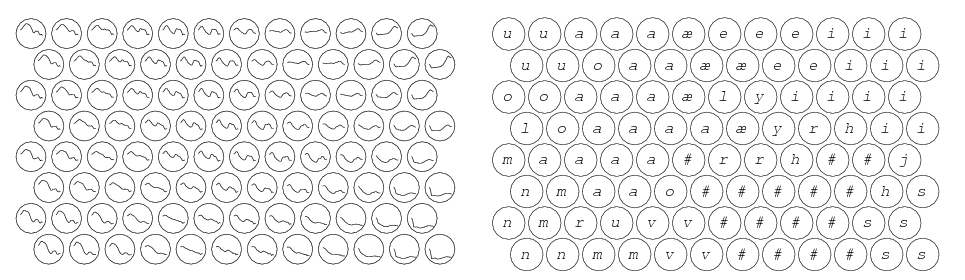
\includegraphics[width=\linewidth]{kohonen_phonemes}
		\caption[Phonème SOM]{Représentation des phonèmes du finnois par la première SOM. A gauche sont représentés les signaux sonores en haute dimension, et à droite leurs phonèmes correspondants. La réduction dimensionnelle provient de l'agencement de ces phonèmes sur la carte. Si ils sont proches entre eux dans leur espace d'entrée (signal), ils seront également proches dans la carte (la position des bulles). \textit{source : scholarpedia}}\label{fig:img:phonemes}

	\end{figureth}

	Le but premier de Kohonen était de présenter un modèle capable de représenter informatiquement l'organisation spatiale des informations dans le cortex humain \cite{kohonen-memory}. 
	
	Il s'inspira pour cela du concept neuroscientifique de colonnes corticales, qui sont un groupe de neurones arrangés verticalement et qui réagissent tous au même stimulus.

\subsubsection{Evolutions et utilisation contemporaine}
	Il y a eu de nombreuses évolutions pendant les presque 40 années d'existence des SOM. En 2002, une bibliographie recensait 5384 articles scientifiques utilisant les SOM \cite{oja2003bibliography}. Ils étaient estimés à plus de 10000 en 2011 \cite{bilbiography-finuni}. Les domaines d'applications sont très variés, allant de l'image et la vidéo, par la parole et le traitement du signal, la médicine et la biologie, l'économie et la finance, de l'urbanisme et d'autres encore. Pour chacun de ces domaines il y a plusieurs types d'utilisations différentes de la SOM. Elle peut par exemple être utilisée en tant que méthode de visualisation capable de rendre humainement interprétable des données à très grande dimension et en les projetant sur des dimensions plus petites. Mais aussi pour faire des traitements sur des données, par exemple pour faire de la classification non supervisée de caractères, de chiffres ou de phonèmes, ou de la détection d'anomalies entre autres. \cite{cottrell2018self} est une revue récente évoquant les aspects les plus importants des SOM et présentant quelques applications typiques. 

	[Evolutions et dérivés.]

\subsection{Principes de fonctionnement}
\subsubsection{Préparation des données}

	Nous présentons dans cette section le fonctionnement de l'algorithme de la SOM que nous avons utilisé. Notre version est tout à fait classique et correspond à ce qui est communément utilisé dans la littérature.\\

	Les données présentées à la SOM doivent être numériques et sous forme de vecteurs. La taille des vecteurs peut être aussi grande que nécessaire, mais toutes les données de la bases doivent avoir la même taille de vecteur. Nous n'avons utilisé que des données normalisées, c'est à dire, dont la valeur est comprise entre 0 et 1 inclus. Par exemple pour apprendre des couleurs avec une SOM, on pourra représenter chaque couleur par un vecteur de taille 3, un élément par composante R,G et B par exemple et renormalisée pour être comprise entre 0 et 1. L'ordre de présentation des vecteur est aléatoire.

\subsubsection{Paramètres}\label{param_som}

	La forme de la SOM dépend de plusieurs paramètres. Le premier est la dimensionalité. Les SOM peuvent aller d'une dimension de un à un nombre arbitrairement grand. Cependant, en pratique elles ne dépassent que rarement deux dimensions. La raison est que la visualisation est plus aisée en deux dimensions pour toutes les applications où cela en est le but premier. C'est aussi la taille idéale pour profiter de la réduction dimensionnelle sans pour autant augmenter de façon exponentielle les coûts en calculs à taille de carte égale. Une carte de 10 neurones de côté aura 100 neurones en deux dimensions et 1000 en 3 dimensions, les coûts en calculs étant proportionnels au nombre de neurones. Nous avons ainsi utilisé exclusivement des cartes bidimensionnelles dans nos expériences. Dans notre cas, nous avons également pris en compte la contrainte matérielle qui rend les toutes les dimensions supérieures à deux difficiles à implémenter efficacement dû à des coûts en communication accrus, car les circuits imprimés sont naturellement en deux dimensions.
	
	Un second choix important est ce que nous appellons la topologie de la SOM. Par topologie, nous entendons la forme des connections entre les neurones qui composent la SOM. Les deux topologies les plus communes pour les SOM sont en grille et hexagonale. Dans la topologie en grille chaque neurone a quatre voisins, un à chaque direction cardinale. En hexagone, chaque neurone a 6 voisins, formant un pavage hexagonal avec les neurones au centre des hexagones. Ces topologies sont deux dimensionnelles, mais il est possible de les rendre toriques ou sphériques. Nous n'explorererons pas cette possibilité dans cette thèse, car cela apporte en général plus de contraintes topologiques, c'est plus difficile pour une sphère de bien couvrir les données que pour une surface plane avec des degrés de libertés au extrémités. D'autres topologies plus exotiques existent et possèdent des propriétés intéressantes \cite{bernard2018np}, cependant nous avons dû nous limiter aux topologies classiques, les différences entre les topologies des SOM n'étant pas notre objet d'étude ici.

	Le dernier type de paramètre pour la SOM sont les paramètres numériques. Il y a parmi ceux-ci : La taille de la SOM, communément notée $n$. Elle défini le nombre de neurones par côté de la SOM. Le nombre total de neurones $N$ est obtenu à partir du carré des côtés : $n^2$. Dans le cas d'une SOM non-carrée, on notera $l$ et $h$ respectivement sa largeur et sa hauteur. Il y a aussi le coefficient d'apprentissage $\epsilon$ (epsilon), défini dans $]0,1[$. Il est décroissant linéairement tout au long de l'apprentissage, On notera dans cette thèse la valeur de départ et la valeur finale, toutes les valeurs intermédiaires seront extrapolées par la droite qui coupe ces deux points en fonction de l'étape courante de l'apprentissage. Le dernier paramètre est le coefficient de voisinage $\sigma$ (sigma), défini dans $[0,1[$. Il sert à définir l'impact des neurones voisins sur les poids du neurone courant. Plus il est élevé, plus les voisins ont un impact et plus la contrainte topologique sera forte. Inversement, une valeur de 0 pour ce paramètre enlève toute contrainte topologique et fait que la SOM se comportera comme un k-means. Comme pour le coefficient d'apprentissage, il décroit linéairement pendant l'apprentissage et nous n'indiquerons que les valeurs de départ et de fin.

\subsubsection{Apprentissage}

	Au début de l'apprentissage, tous les poids des neurones sont initialisés aléatoirement entre 0 et 1. L'apprentissage dure un certain nombre d'époques définies avant lancement. Une époque contient exactement le nombre d'itérations requises pour que chaque élément de la base d'apprentissage soit utilisé exactement une seule fois par époque. Lors d'une itération, on sélectionne aléatoirement un vecteur d'apprentissage parmi la base d'apprentissage, qui n'a pas déjà été utilisé lors de cette époque. 

	Une itération se déroule en deux étapes : 
	\begin{itemize}
		\item La phase de recherche, qui consiste à trouver la \textit{Best Matching Unit} (BMU) parmi tous les neurones. Elle correspond au neurone qui a la plus petite distance $L^2$ (distance euclidienne), entre ses poids et le vecteur d'apprentissage.
		\item La phase d'adaptation, qui modifie les poids des neurones selon l'équation suivante :
		\begin{equation}\label{eq:SOM}
			w_i(t+1) = w_i(t)+\epsilon(t)\cdot\Theta(\sigma(t),d_{i,bmu})\cdot(v-w_i(t))
		\end{equation} avec $i$ le neurone courant, $w_i$ les poids de ce neurone, $t$ l'itération courante, $\epsilon$ et $\sigma$ des paramètres de la SOM définis dans la section \ref{param_som}. $d_{i, bmu}$ est la distance $L^1$ (distance de manhattan) normalisée entre le neurone $i$ et la BMU. $\Theta$ est une fonction gaussienne centrée normalisée d'écart type $\sigma$. $v$ est la vecteur d'apprentissage.
	\end{itemize}

	On répète ces deux étapes jusqu'à ce que l'on finisse la dernière époque, est l'apprentissage sera terminé.

\subsubsection{Reconstruction}
	
	On appelle reconstruction le fait de remplacer un ensemble de vecteurs, de longueur similaire à ceux sur laquelle la SOM a été apprise, par les poids des neurones les plus proches.

	Cette reconstruction est par exemple utilisée pour de la compression de données, car à la place de mémoriser un ensemble de vecteurs, il n'y a besoin que de mémoriser les poids de la SOM et l'indice de chaque neurone le plus proche de chaque vecteur de l'ensemble. Cette compression est avec perte, du fait que les poids des neurones sont en général pas exactement les mêmes que les vecteurs présentés, même lorsque ceux-ci faisaient partie de la base d'apprentissage.

	\subsection{Gaz Neuronaux en Expansion}

	Bien que nos travaux se soient focalisés sur les cartes auto-organisatrices, notre approche se veut généraliste et transposable à d'autres modèles de quantification vectorielle avec topologie. Nous avons souhaité valider expérimentalement cette transposition en utilisant les Gaz neuronaux en expansion. C'est un autre modèle similaire aux SOM mais avec une approche tout à fait différente sur la topologie, qui devient dynamique et non pas fixe. 

	\subsubsection{Développements}

	Une évolution majeure inspirée par les carte auto-organisatrices a été le développement des différents types de gaz neuronaux (Neural Gases, NG), qui a commencé avec \cite{martinetz1991neural}, en tant qu'alternative aux k-means car ils ne disposent pas de topologie non plus. Puis ce sont les Gaz Neuronaux en Expansion (Growing Neural Gases, GNG) \cite{fritzke1995growing} qui ont sensiblement amélioré l'approche en ajoutant un mécanisme de croissance qui ajoute des neurones lors de l'apprentissage et une topologie avec des connexions qui se créent et qui disparaissent entre les neurones.

	De nos jours, plusieurs variantes des GNG existent qui améliorent certains aspects de cet algorithme. Notablement, Growing when required \cite{marsland2002self} adapte la croissance du nombre de neurones en fonction de ce que le réseau à déjà appris, produisant une forte neurogénèse au début de l'apprentissage et une stabilisation une fois que les données ont été suffisament apprises. Une autre variante sont les Icremental growing neural gases \cite{prudent2005incremental}. Ils permettent d'apprendre de nouvelles données sans oublier les anciennes en combinant plasticité et stabilité.

	Pour la suite, nous avons décidé d'utiliser uniquement l'algorithme des Gaz neuronaux en expansion. C'est le plus utilisé, et les avantages qu'apportent les variants ne sont pas nécessaires dans notre cas.

	\subsubsection{Fonctionnement}

	Nous ne présenterons le fonctionnement que des gaz neuronaux en expansion. L'algorithme ne se réduisant pas aisément en quelques formules, nous prendrons une approche itérative, similaire à celle que l'on peut trouver dans l'article original, pour expliquer les différents mécanismes à l'oeuvre.\\

	Une itération se décompose en 9 étapes :
	\begin{enumerate}
		\item Choisir au hasard un élément de la base d'apprentissage parmi ceux qui n'ont pas déjà été tirés lors de cette époque.
		\item Trouver les deux neurones les plus proches : $s_1$ et $s_2$.
		\item Incrémenter l'âge des synapses de tous les voisins topologiques directs de $s_1$.
		\item Ajouter la distance euclidienne au carré entre le vecteur d'apprentissage et $s_1$ à la variable d'erreur de $s_1$.
		\item Mettre à jour les poids de $s_1$ et de tous ces voisins topologiques directs $s_n$. Les formules sont :
		\begin{equation}
			w_{s_1}(t+1) = w_{s_1}(t) + \epsilon_{\textit{bmu}} \times (v - w_{s_1}(t))
		\end{equation}
		\begin{equation}
			w_{s_n}(t+1) = w_{s_n}(t) + \epsilon_{n} \times (v - w_{s_n}(t))
		\end{equation}
		\item Si $s_1$ et $s_2$ sont voisins topologiques directs, mettre à jour l'âge de la synapse à 0. Sinon créer une synapse.
		\item Enlever toutes les synapses avec un âge supérieur à $a_{\textit{max}}$. Si des neurones se retrouvent sans synapses, les enlever aussi.
		\item Si l'itération courante est un multiple de $\lambda$, insérer un nouveau neurone comme suit :
		\begin{itemize}
			\item Trouver le neurone avec l'erreur la plus élevée $q$.
			\item Créer un nouveau neurone $r$ à distance égale de $q$ et de son voisin direct avec l'erreur la plus élevée $f$.
			\begin{equation}
				w_r(t+1) = \frac{w_q(t) + w_f(t)}{2}  
			\end{equation}
			\item Ajouter des synapses d'âge 0 entre $r$ et $q$ ainsi qu'entre $r$ et $f$. Enlever la synapse entre $q$ et $f$.
			\item Réduire l'erreur de $q$ et $f$ en la multipliant par une constante $\alpha$. Initialiser l'erreur de $r$ avec la nouvelle valeur de l'erreur de $q$.
		\end{itemize}
		\item Réduire toutes les variables d'erreur en les multipliant par une constante $d$.
	\end{enumerate}\text{\\}

	L'apprentissage s'arrête au bout d'un certain nombre prédéfini d'époques, comme pour la SOM. L'effet de chaque paramètre peut être compris aisément par le contexte dans lequel il est utilisé, ainsi nous n'irons pas de le détail de chacun d'entre eux. Le paramètre $\lambda$, ajustant la vitesse de création de nouveaux neurones, sera fixé de telle sorte qu'à la fin de l'apprentissage il y ait le même nombre de neurones dans le GNG que dans la SOM à laquelle on souhaite se comparer. La reconstruction se passe de la même façon que pour la SOM. Les valeurs que l'on aura utilisées pour nos paramètres sera précisée dans la section expérimentale correspondante.

	\subsection{DNF}\label{sec:sota:dnf}
	

	Following the seminal work of \cite{Fix:dnf:2011}, we choose to couple our autonomous novelty detection tool to a robust bio-inspired tracking technique based on Dynamic Neural Fields (DNF). DNF are populations of partial differential equations first mathematically analyzed by \cite{amari:dnf:1977} in a continuous framework. We use a discrete DNF built from populations of excitatory and inhibitory neurons that interact continuously, with a on-center off-surround approach modeled as a synaptic kernel computed as a difference of gaussians applied to the distance between neurons in the neural map. These DNF have been successfully applied to sequential visual exploration of an environment \cite{Fix:dnf:2011} or in \cite{rougier:attention:2005}, with great robustness properties that can even improve with some adaptation like the use of simple spiking neurons \cite{vazquez:dnf:2011}. 

	\subsubsection{Fonctionnement}

	Continuous Neural Fields Theory (CNFT) has lead to the development of two dimensional Dynamic Neural Fields (DNF) \cite{Taylor2D}. Neural fields are models that represent the evolution of a population of neurons. In our case, we use a two dimensional DNF. The number of neurons is dependent and equal to the size of the input map, because neurons are connected in a retinotopic way to afferent inputs, and are connected in an all-to-all connection scheme between them. All neurons also have a real value attached to them that we call potential. This potential $u(x,t)$, with $x$ being the neuron position in the field and $t$ the time of the simulation, is ruled by the following differential equation :

$$\tau \frac{\partial u(x, t)}{\partial t} = -u(x,t)+\int u(x',t)\omega(||x-x'||)\delta y + \text{Input}(x,t)$$

With :
\begin{itemize}
    \item $\tau$ is the time constant.
    \item $-u(x,t)$ is the decay term. It is meant to suppress already activated neurons when there is no input or lateral excitation.
    \item $\omega(||x-x'||)$ is the lateral interaction. It represents the effect of the other neurons onto this neuron's potential. We are using a difference of gaussian with the excitatory gaussian part being narrow with high intensity and the inhibitory one being wide with low intensity. This leads to close neurons having an excitatory effect onto each other and far away neurons inhibiting themselves.
    \item $Input(x,t)$ is the current value of the afferent input extracted from the input map for this neuron.
\end{itemize}

For the sake of simplicity and computability, we implement a spatially and temporaly discretized version of the previous formula. It is obtained by handling potentials of a discrete set of neurons (neural map instead of neural manifold) and by using a simple Euler method to estimate the state of $u(x,t+\Delta t)$ knowing $u(x,t)$:

$$u(x, t+\Delta t) = u(x, t) +\frac{\Delta t\left(-u(x, t)+\sum u(x', t)\omega(||x-x'||) + \text{Input}(x, t+\Delta t)\right)}{\tau}$$

$\Delta t$ is the time step between two estimations, it can be the same for all neurons (synchronous) or different each time (asynchronous). It should be noted that in the original DNF formula, there are more parameters such as resting potential but since we do not use them here, we did not mention them.

It is often difficult to understand how a DNF will behave just from the formula. We have set it up with optimized parameters in order to have a winner-takes-all behaviour where the most prominent and spatially coherent features in the input map create a local bubble of activation in the neural map and suppress the ability of other such bubbles to appear elsewhere in the map. 

\bibliographystyle{francaissc}
\bibliography{Chapitre1/Biblio}